\documentclass[twoside,12pt]{article}

\usepackage{dsctemplate}
\usepackage[margin=1in]{geometry}
\usepackage{amsmath}
\usepackage{amssymb,amsthm}
\usepackage{fancyhdr}
\usepackage{nicefrac}
\usepackage{minted}
\usetikzlibrary{quotes,angles,positioning,arrows.meta}
\usetikzlibrary{calc}
\usepackage{enumitem}
\usepackage{fancyvrb}
\usepackage{dirtytalk}


\DefineVerbatimEnvironment{verbatim}{Verbatim}{xleftmargin=.5in}

% \renewcommand{\rmdefault}{phv} % Arial
% \renewcommand{\sfdefault}{phv} % Arial

% configuration
% ------------------------------------------------------------------------------

% control whether solutions are show or hidden
\showsolntrue

% page headers only on odd pages
\pagestyle{fancy}
\fancyhead{}
\fancyhead[RO]{PID or Name: \rule{3in}{.5pt}}
\renewcommand{\headrulewidth}{0pt}

% ------------------------------------------------------------------------------

\begin{document}

\thispagestyle{empty}

\begin{center}
    \noindent \textbf{\large{Data Overview: Fraudulent Transactions}} 
\end{center}

\vspace{.25in}

\noindent Today, we're diving into the high-stakes world of fraud detection. Each row in the DataFrame \texttt{txn} represents one online transaction, or purchase. The \texttt{txn} DataFrame is indexed by \texttt{"transaction\_id" (int)}, which is a unique identifier for a transaction. The columns of \texttt{txn} are as follows:
\begin{itemize}
    \item \texttt{"is\_fraud" (bool)}: \texttt{True} if the transaction was fraudulent and \texttt{False} if not.
    \item \texttt{"amount" (float)}: The dollar amount of the transaction.
    % \item \texttt{"product\_code" (str)}: A code for the product purchased in the transaction; either \texttt{"H"} for household, \texttt{"C"} for consumer goods, \texttt{"S"} for services, or \texttt{"R"} for recreation.
    \item \texttt{"method" (str)}: The payment method; either \texttt{"debit"} or \texttt{"credit"}.
    \item \texttt{"card" (str)}: The payment network of the card used for the transaction; either \texttt{"visa"}, \texttt{"mastercard"}, \texttt{"american express"}, or \texttt{"discover"}.
    % \item \texttt{"three\_days" (int)}: The number of transactions made by the card in the last three days.
    \item \texttt{"lifetime" (float)}: The total transaction amount of all transactions made with this card over its lifetime.
    \item \texttt{"browser" (str)}: The web browser used for the online transaction. There are 100 distinct browser types in this column; some examples include \texttt{"samsung browser 6.2"}, \texttt{"mobile safari 11.0"}, and \texttt{"chrome 62.0"}.
    % \item \texttt{"device\_type" (str)}: The type of device used for the online transaction; either \texttt{"mobile"} or \texttt{"desktop"}.
    
\end{itemize}
\vspace{.2in}

\noindent The first few rows of \texttt{txn} are shown below, though \texttt{txn} has 140,000 rows in total. Assume that the data in \texttt{txn} is a simple random sample from the much larger population of \textbf{all} online transactions.


\begin{center}
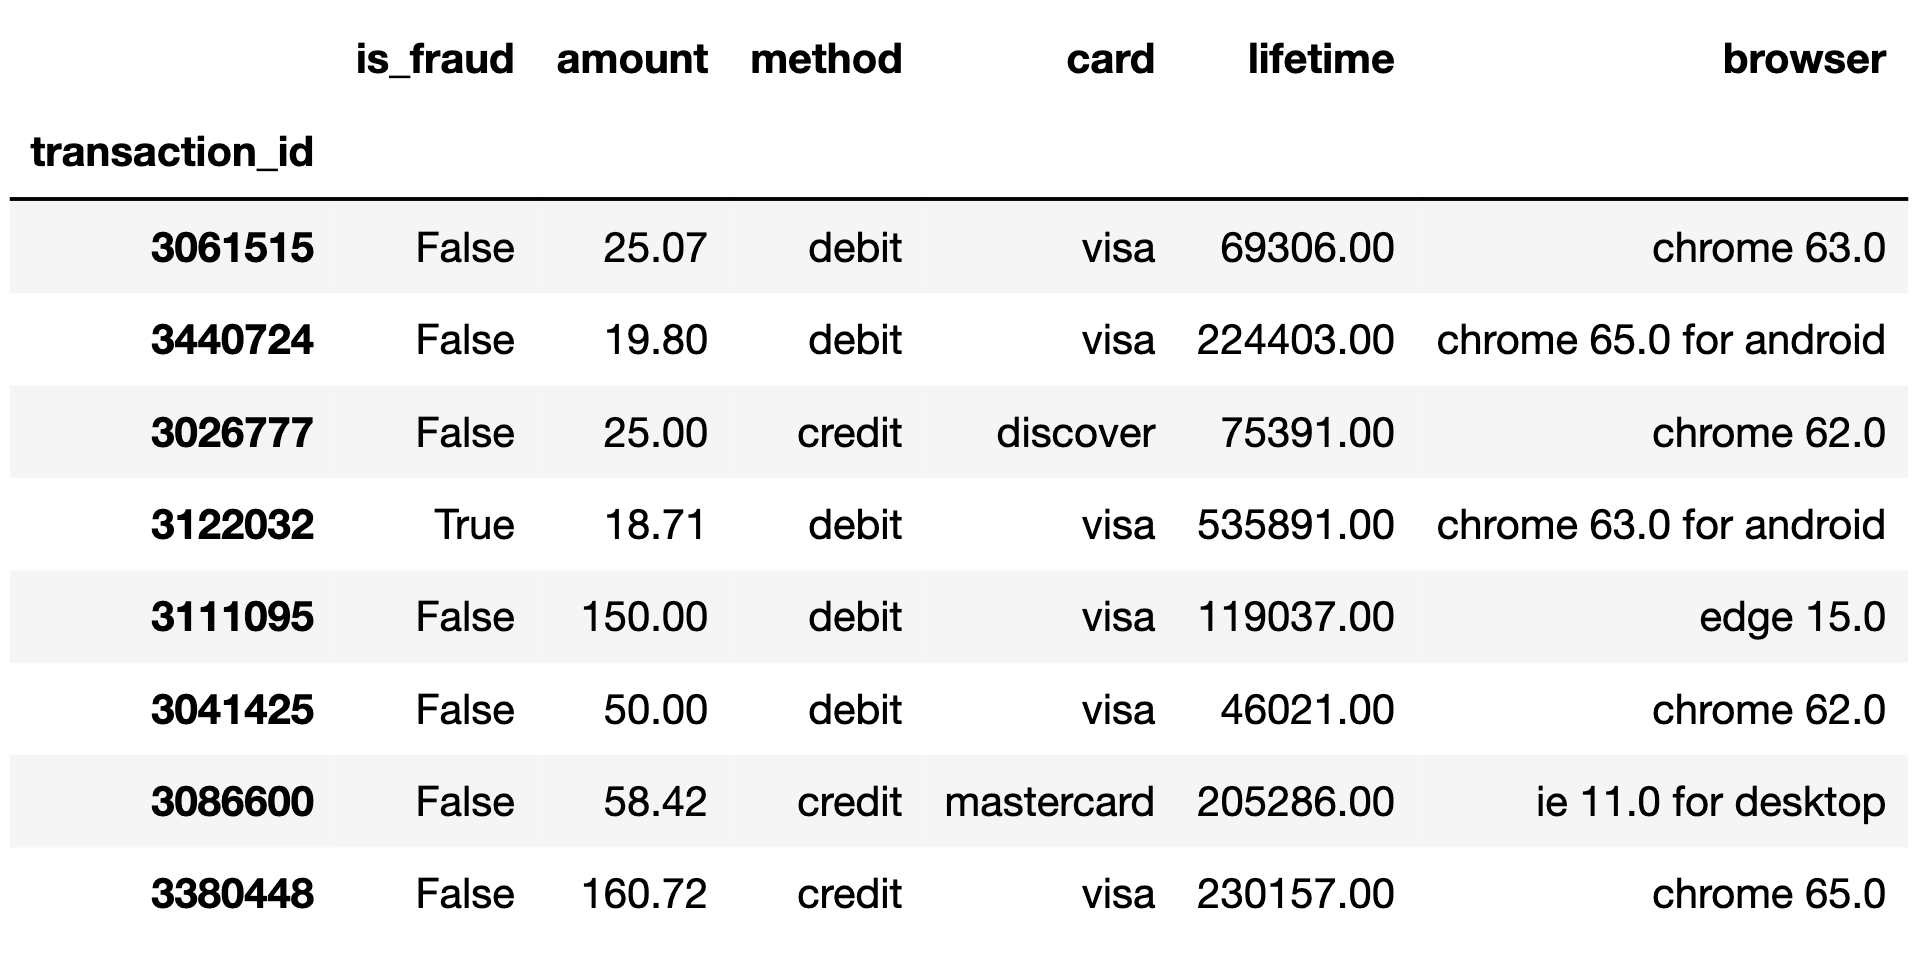
\includegraphics[width=0.9\textwidth]{final_images/final-data-info.png}
\end{center}

\noindent Throughout this exam, assume that we have already run \texttt{import babypandas as bpd} and \texttt{import numpy as np}.


\end{document}
